\section{Introduction}

A spherical robot in the style of the BB-8 toy hides its drive inside the shell: a two-wheel
cart rolls on the inner surface like a hamster in a ball \cite{chase2012spherical,halme1996spherical}.
We ask whether such a robot can follow a walking person who carries nothing but a phone, using
sound. The phone repeats a 10\,ms linear chirp every 50\,ms near or above the edge of human
hearing, and a four-microphone array (INMP441-class MEMS microphones, 5\,cm radius) on the
robot's levelled mast estimates the bearing and range of the phone. The robot then has to
drive toward the person across flat ground, slopes, rough ground, grass, a reverberant room
and an obstacle field.

The task combines two hard parts. Acoustically, the band that keeps the beacon inaudible
(17--23\,kHz) has wavelengths of 15--20\,mm, so a 5\,cm array is spatially aliased: each
microphone-pair phase difference maps to several candidate directions, and ground reflections,
walls and obstacles add coherent copies of the chirp. Mechanically, a pendulum-cart sphere
is underactuated, lags its commands, drifts downhill on slopes and loses speed on grass.

We built a simulator for both parts and compared, on identical scenarios, (i) a deep
multichannel localizer feeding a Kalman tracker and a pursuit law, (ii) a reinforcement-learning
policy (PPO), and (iii) a cascaded PID controller driven by the deep localizer with a learned
terrain residual, against a classical GCC-PHAT/SRP-PHAT localizer \cite{knapp1976gcc,dibiase2001srp}
and an oracle with true bearing and range. Everything reported here is simulation;
we built the ESP32 firmware and a companion app, but no hardware experiment was run.

\textbf{Contributions.} (1) A GPU acoustic renderer with exact fractional delays, image-source
multipath, obstacle scattering and occlusion, and two front-end models: an idealised transducer
and a realistic phone-speaker plus INMP441 chain. (2) A localizer that starts from a
physics-initialised steering layer over band-masked STFT cross-spectra and learns which frames
to trust, with a documented account of two designs that failed. (3) A closed-loop comparison of
six controllers on six terrains with per-episode metrics and confidence intervals. (4) Firmware
and a companion app that implement the same packet protocol, tested against software stand-ins.

\section{Related work}

\textbf{Time-delay and steered-response localization.} Knapp and Carter's generalized
cross-correlation with the phase transform (GCC-PHAT) \cite{knapp1976gcc} whitens the
cross-spectrum so that every frequency contributes equally to the delay estimate; steered
response power with PHAT (SRP-PHAT) sums these over microphone pairs on a grid of candidate
directions and is a standard robust baseline in reverberant rooms \cite{dibiase2001srp}. Our
classical baseline is exactly this: SRP-PHAT over 360 azimuths and 13 elevations, pairwise
GCC-PHAT with a least-squares direction fit, and matched-filter time-of-flight ranging.

\textbf{Acoustic localization with phones.} Daredevil \cite{constandache2014daredevil} localizes
phones indoors using sound and microphone arrays; MilliSonic \cite{wang2019millisonic} tracks a
device with near-ultrasonic FMCW signals and reports sub-millimetre one-dimensional accuracy by
exploiting carrier phase. Both systems were evaluated on real hardware. Our setting differs (a
moving, tilting, self-propelled receiver on varied terrain, a single small array, and pulsed
chirps) and our results are simulated; we do not claim parity with either system, and nothing
here approaches MilliSonic's accuracy.

\textbf{Learned sound source localization.} Convolutional-recurrent networks on multichannel
spectrograms with phase or inter-channel features are now common for direction of arrival
estimation \cite{adavanne2019seld,chakrabarty2019doa}; see \cite{grumiaux2022survey} for a survey.
Our localizer belongs to this family. It differs in that its first layer is initialised to the
SRP-PHAT beamformer of the actual array geometry, which we found necessary at this aperture and
frequency.

\textbf{Spherical robots and learned control.} Pendulum-driven spheres and their dynamics are
reviewed in \cite{chase2012spherical}; early motion control work includes
\cite{halme1996spherical}. Combining a model-based controller with a learned correction has been
studied as residual reinforcement learning \cite{johannink2019residual}; our residual is
simpler, a supervised inverse-dynamics correction to the PID's feedforward. The policy is trained
with PPO \cite{schulman2017ppo} in Stable-Baselines3 \cite{raffin2021sb3}.

\section{Method}

\subsection{Acoustic simulation}

Each 50\,ms control step renders one chirp at 48\,kHz into a 2048-sample (42.7\,ms) window per
microphone, starting at the assumed emission time. Propagation paths are: the direct path
(attenuated by 8--20\,dB per obstacle that occludes it), a ground image (reflection coefficient
by terrain, from 0.6--0.9 on flat ground to 0.05--0.3 on grass), an optional outdoor facade
image, scattering from up to 8 cylindrical obstacles, and indoors the shoebox image sources up
to second order \cite{allen1979image} plus a 24-path diffuse tail. Each path has a per-microphone
length; the delay uses a temperature-dependent speed of sound (5--35\,$^\circ$C) and is applied
exactly as a linear phase in a 4096-point FFT over 16--23.8\,kHz, so sub-sample delays are not
quantised. Spherical spreading, air absorption (0.55\,dB/m) and terrain excess attenuation
(0.5--1.5\,dB/m on grass) set amplitudes. The receiving array may be tilted: the head follows a
quarter of the cart's lean (an assumed passively levelled mast).

Two front-end channels are simulated. \emph{Channel A} (\texttt{A\_us}) is an ideal transducer
and flat microphone with the 20--22.5\,kHz chirp. \emph{Channel B} applies a phone-speaker
roll-off (fourth order, corner 18.5--21\,kHz), a second-order MEMS roll-off at 19\,kHz and a
model of the INMP441 decimation filter (pass band to $0.423f_s$, stop band from $0.5f_s$; the
exact edges are to be confirmed against the data sheet \cite{inmp441}), plus per-microphone gain
($\pm$1\,dB) and delay ($\pm$2\,$\mu$s) mismatch. Channel B is used with the 20--22.5\,kHz chirp
(\texttt{B\_us}; mean in-band gain \FeBus\,dB at a 20\,kHz speaker corner) and with a 17--19.5\,kHz fallback chirp
(\texttt{B\_fb}; \FeBfb\,dB), which is what real hardware would likely need. White noise is added at the
digital output with a direct-path SNR at 1\,m drawn from 10--45\,dB, and a random overall gain
of $\pm$6\,dB.

\textbf{Range needs synchronisation.} Time of flight is observable only because we assume the
phone emits on a schedule the robot knows. We model the residual error of such a sync as
100\,$\mu$s per-chirp jitter plus a per-episode bias of up to $\pm$200\,$\mu$s (up to 7\,cm).
Without it, only bearing and a weak level cue would remain.

\subsection{Robot and terrain}

The sphere ($R=0.2$\,m, shell 1.0\,kg) contains a pendulum cart (1.5\,kg, centre of mass 0.1\,m
below the centre) with two wheels driven by DC motors modelled by a linear torque--speed curve
from a duty cycle $u\in[-1,1]$. Pitch dynamics follow a planar Lagrangian sphere--pendulum model
with rolling without slip; a passive lateral pendulum gives roll and downhill drift on slopes;
yaw follows first-order dynamics from differential torque. Rolling resistance, drag and yaw
damping are terrain dependent and randomised by $\pm$15\%. Physics runs at 200\,Hz and control
at 20\,Hz (one chirp per decision). Steady speed at full duty is \VFlatFull\,m/s on flat ground, \VUphillEightFull\,m/s up an
8$^\circ$ slope and \VGrassFull\,m/s on grass (\texttt{results/sanity.json}). The terrains are \emph{flat}, \emph{slope} (5--10$^\circ$),
\emph{rough} (random height field), \emph{grass} (high resistance, absorptive ground),
\emph{indoor} (rooms of 4--10\,m in the dataset and 6--10\,m in closed loop, with reverberation;
walls block motion) and \emph{obstacles}
(posts that block motion, scatter sound and occlude the direct path). The person follows a
scripted walk. For each terrain the same seeded scenarios are replayed for
every controller.

\subsection{Deep localizer}

\textbf{Input.} A 256-point STFT (hop 32) of each channel, restricted to the 32 bins from 16.9 to
22.9\,kHz and 65 frames. The 18 input channels are 4 normalised log-power maps; the real and
imaginary parts of the cross-spectrum $G_{ij}(f,t)=X_i X_j^*$ for all six microphone pairs,
divided by $\sum_t |G_{ij}(f,t)|$ and zeroed outside the known chirp band; a time ramp (time
since emission, which carries range) and a frequency ramp. The per-frequency normalisation is a
time--frequency analogue of PHAT: every in-band frequency gets equal total weight while frames
keep their relative energy, so the network can still tell early from late arrivals. The chirp
band is a system setting known to the receiver; the classical baseline uses the same mask.

\textbf{Architecture} (\TrainFullParams{} parameters). A steering layer maps the 12 phase
channels, per frequency, to 504 beam directions (72 azimuths $\times$ 7 elevations,
0--60$^\circ$) and sums over frequency, producing a beam--time map of $7\times72\times65$. Its
weights are initialised to the SRP-PHAT steering vectors of the array and remain trainable.
Three residual convolution blocks with circular padding in azimuth process the beam maps
(spatial branch, 32 channels at full resolution). Four residual convolution blocks with
frequency pooling process log-power and the ramps (spectral branch). Per frame, the spatial
branch's azimuth-max and azimuth-mean summaries and the spectral features are projected to 256
dimensions and passed through a two-layer bidirectional GRU (192 units per direction). Two
attention heads over the 65 frames then pool (a) the spatial feature maps, modulated by the GRU
context (FiLM), into 72 azimuth logits through two circular 1-D convolutions, and (b) the GRU
states into a range mean and log-variance. The frame attention lets the network favour the
direct-path frames over later echoes, in the spirit of the precedence effect
\cite{litovsky1999precedence}, which a full-window SRP-PHAT cannot do.

\textbf{Loss and training.} Cross-entropy against a Gaussian-smoothed (5$^\circ$) azimuth target,
plus smooth-L1 and Gaussian negative log-likelihood on range. AdamW, one-cycle learning rate
(peak $10^{-3}$), batch \BatchSize, \TrainFullEpochs{} epochs, fp16 mixed precision on an
\GPU{}, model selection on the validation set. Each batch applies one of the 8 exact symmetries
of the square array (a microphone permutation with the matching azimuth rotation or
reflection), checked against SRP-PHAT, which gives identical errors under all 8 transforms.

\textbf{Design history.} Two earlier designs that fed per-bin unit phasors to a 2-D CNN with a
recurrent head plateaued at \AbortOneValMAE$^\circ$ and \AbortTwoValMAE$^\circ$ validation MAE
(chance: 90$^\circ$) and were stopped after \AbortOneEpochs{} and \AbortTwoEpochs{} epochs. With
spatial aliasing the phase-to-direction map differs per frequency, which a convolution shared
across frequency cannot represent. A diagnostic (\texttt{scripts/debug\_steer.py}) showed that a
fixed steered response over the STFT matches the classical baseline only with equal per-frequency
weighting \emph{and} out-of-band masking, which led to the current input and steering layer. The
current design without symmetry augmentation overfit (train \NoAugTrainMAE$^\circ$ vs.\
validation \NoAugValMAE$^\circ$ MAE after \NoAugEpochs{} epochs, stopped). All histories are in
\texttt{results/} and in Fig.~\ref{fig:history}.

\textbf{Ablations.} \emph{Magnitude only}: the phase channels and the spatial branch are
removed; azimuth logits come from the GRU summary. \emph{No multipath in training}: the same
model trained on an anechoic copy of the training set (direct path only), tested on the normal
test set.

\subsection{Controllers}

All controllers output wheel duties $(u_L,u_R)$, which is what the firmware receives.

\textbf{Tracker and pursuit} (\emph{GCC-PHAT + tracker}, \emph{DL + tracker}). A constant-velocity
Kalman filter \cite{kalman1960} tracks the person in the robot's dead-reckoning frame (wheel
odometry and gyro). Measurement noise comes from the localizer: the DL net's predicted azimuth
spread and range variance, or for the classical baseline a heuristic from the SRP peak height.
Gating rejects outliers and the track re-initialises after 10 consecutive rejections. A pursuit
law sets the yaw-rate command proportional to bearing and the speed command proportional to
range error beyond the 0.8\,m standoff, plus the tracked person's radial speed as feedforward;
a nominal mixer converts $(v,\omega)$ into duties.

\textbf{DL + PID.} The same tracked estimate drives an outer PID on bearing and range that sets
$(v^*,\omega^*)$, and an inner PI on measured speed and yaw rate (wheel odometry, gyro) that
corrects the nominal mixer's duties.

\textbf{DL + PID + residual.} What the residual learns is a supervised inverse-dynamics map
$u_t = f(h_t, v_{\mathrm{target}}, \omega_{\mathrm{target}})$, where $h_t$ is the last 0.5\,s of
applied duties and noisy proprioception (speed, yaw rate, pitch, pitch rate, roll), and the
targets are the speed and yaw rate measured 0.2\,s after $u_t$ is applied. It is trained on
random piecewise-constant commands on all six terrains, sampled only at command switches (an MLP,
72$\to$128$\to$128$\to$2, \ResEpochs{} epochs; validation duty MAE \ResValMAE{} against
\ResMixerMAE{} for the flat-ground mixer). At run time it is queried at the \emph{measured} motion,
and the residual added to the PID's feedforward $\mathrm{mix}(v^*,\omega^*)$ is
$f(h,v,\omega)-\mathrm{mix}(v,\omega)$, clipped to $\pm0.5$: the extra duty needed to hold the
current motion on the terrain implied by recent history (more uphill or on grass, less downhill).
It sees neither the terrain label nor any acoustic input.

Our first residual got two things wrong, and both are instructive. Sampling every step of
each held command let the network copy the previous duty, which is part of its input (validation
MSE \ResOldValMSE, an illusion; \texttt{results/superseded\_residual\_v1.json}). Querying it at the PID setpoint turned it into a second
high-gain speed loop. Together they saturated the wheels and tumbled the cart even with oracle
localization (\texttt{scripts/debug\_pid.py}); the version described above fixes both.

\textbf{RL (PPO).} Observation: four stacked frames of 24 values, namely 17 classical acoustic
features (six GCC-PHAT lags and peak heights, SRP-PHAT azimuth as cosine and sine, SRP peak,
matched-filter range, level), 5 proprioceptive values and the previous action. The policy is not
given the deep localizer; this keeps the RL observation cheap enough for millions of steps, and
it is a confound in the comparison (Sec.~\ref{sec:discussion}). Action: duties. Reward per step:
$+5\,(d_{t-1}-d_t)$ while beyond the standoff, $-0.05\max(d-0.8,0)$, $+0.1$ within the
\FollowRadius\,m follow radius, $-0.02\,\dot\psi^2$, $-0.05\,\lVert u_t-u_{t-1}\rVert^2$, $-0.5$
closer than 0.4\,m, $-1$ per collision, $-0.05$ per step while stuck, and $-10$ with termination
on a tumble (the cart looping inside the shell) or if the person is more than 12\,m away. The
true distance $d$ is privileged and used only in the reward. PPO with 32 parallel environments
(terrain sampled at every reset, 30\,s episodes), 256-step rollouts, batch 1024, 8 epochs, learning
rate $3\cdot10^{-4}$, two 256-unit hidden layers.

\section{Experimental setup}

\textbf{Data.} \NTrainSet{} training, \NValSet{} validation and \NTestSet{} test recordings (plus
an anechoic copy of the training set, \NAnechoicSet), each with a uniformly random terrain,
azimuth, horizontal range (0.5--7\,m), phone height (0.75--1.45\,m), head tilt, temperature,
SNR, sync error and channel (A\_us 50\%, B\_us 15\%, B\_fb 35\%). Splits use disjoint seeds.

\textbf{Localization metrics.} Absolute azimuth error (MAE, RMSE, median, 90th percentile,
fraction below 10$^\circ$) and horizontal range error, on the full test set, for every method on
the same recordings.

\textbf{Closed-loop protocol.} For each terrain, $N$ seeded 60\,s episodes (identical for all
controllers) start with the person 2--4\,m away in a random direction; the person walks at
0.25--0.85\,m/s with random turns and pauses (15\% of segments), around walls and obstacles. An episode is a
\emph{success} if, after a \WarmupS\,s warm-up, the robot stays within \FollowRadius\,m of the
person for at least \SuccessFrac\% of the time and never tumbles. We also report mean distance
after warm-up, final distance, time to first reach the radius, path length, control effort
(mean $u^2$), collisions, tumbles, and time closer than 0.4\,m. Intervals are 95\% normal
intervals over episodes.

\textbf{Compute.} All training and evaluation ran on one \GPU{} (8\,GB) with PyTorch
\TorchVersion{} (CUDA 12.8); the PPO policy network ran on the CPU while the environments
rendered audio on the GPU.

\section{Results}
\label{sec:results}

Every number in this section is read from \texttt{results/*.json} by
\texttt{scripts/paper\_tables.py}, and every figure is drawn from the same files by
\texttt{scripts/make\_figures.py}.

\subsection{Training}

The localizer trained for \TrainFullEpochs{} epochs in \TrainFullMinutes{} minutes on the
\GPU{} (Fig.~\ref{fig:trainloc}). Its best validation epoch was the last one
(\TrainFullBestEpoch), so it had not fully converged. The design history
(Fig.~\ref{fig:history}) shows why the final input and steering layer were needed: both earlier
designs stayed near \AbortOneValMAE$^\circ$ MAE, and the final design without symmetry
augmentation overfit within \NoAugEpochs{} epochs.

PPO ran for \RLSteps{} environment steps in \RLHours{} hours (Fig.~\ref{fig:trainrl}). The mean
episode return rose from \RLFirstReturn{} to about \RLFinalReturn{} (mean of the last 5\% of
updates) and was flat for the last half of training. This is the third attempt. The first
crashed early in training (its log was overwritten, so we do not report its step count), and the
second crashed at \RLCrashTwoSteps{} steps. Both crashes were CUDA errors raised when another GPU
process on the same Windows machine started or exited. The third run
saved a checkpoint every 250{,}000 steps but was not interrupted. The curve of the second run is
kept in \texttt{results/crashed\_rl\_run2\_curve.json}.

The residual network reached a validation duty MAE of \ResValMAE{} over \ResNTrain{} training
samples, against \ResMixerMAE{} for the flat-ground mixer it corrects
(Fig.~\ref{fig:trainres}).

\begin{figure*}[t]
\centering
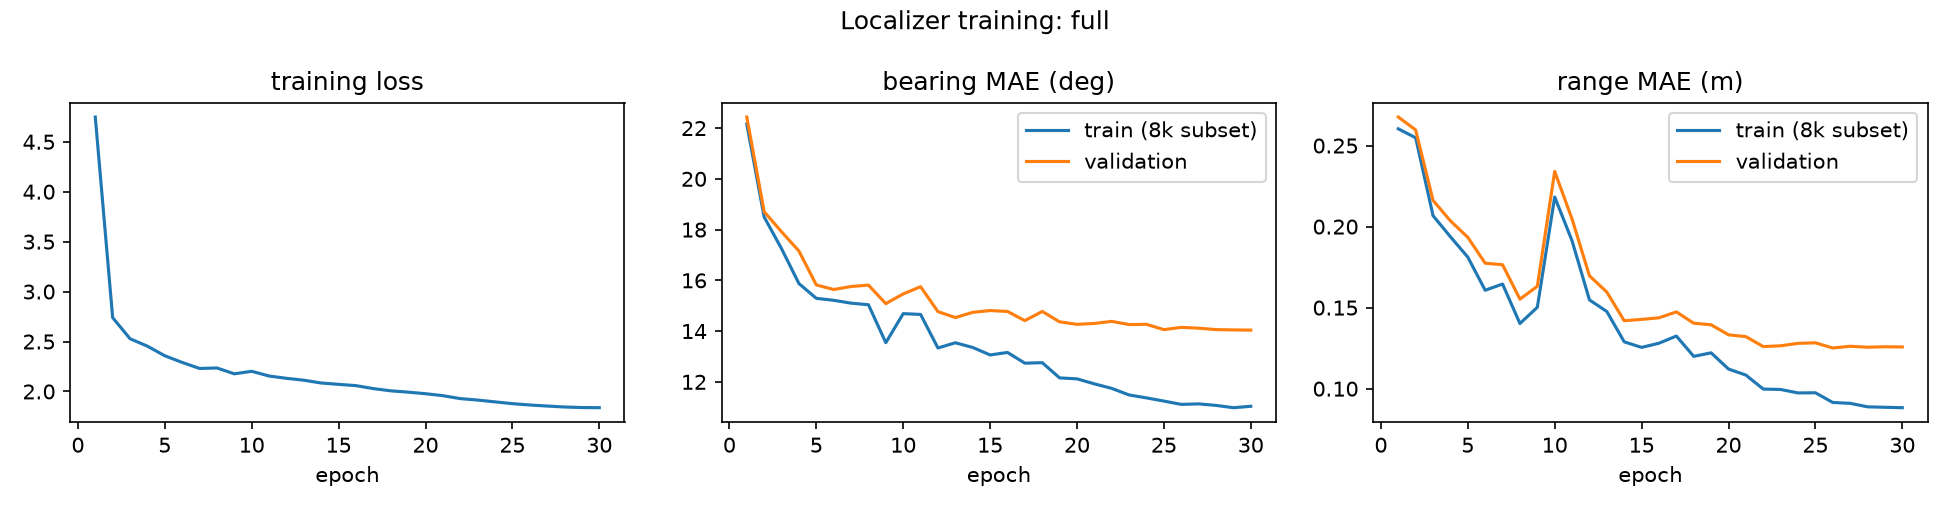
\includegraphics[width=\textwidth]{train_localizer_full.png}
\caption{Localizer training (\TrainFullNTrain{} examples, batch \BatchSize, fp16 on the \GPU).
The training curve is measured on a fixed 8{,}000-example subset with augmentation off.}
\label{fig:trainloc}
\end{figure*}

\begin{figure*}[t]
\centering
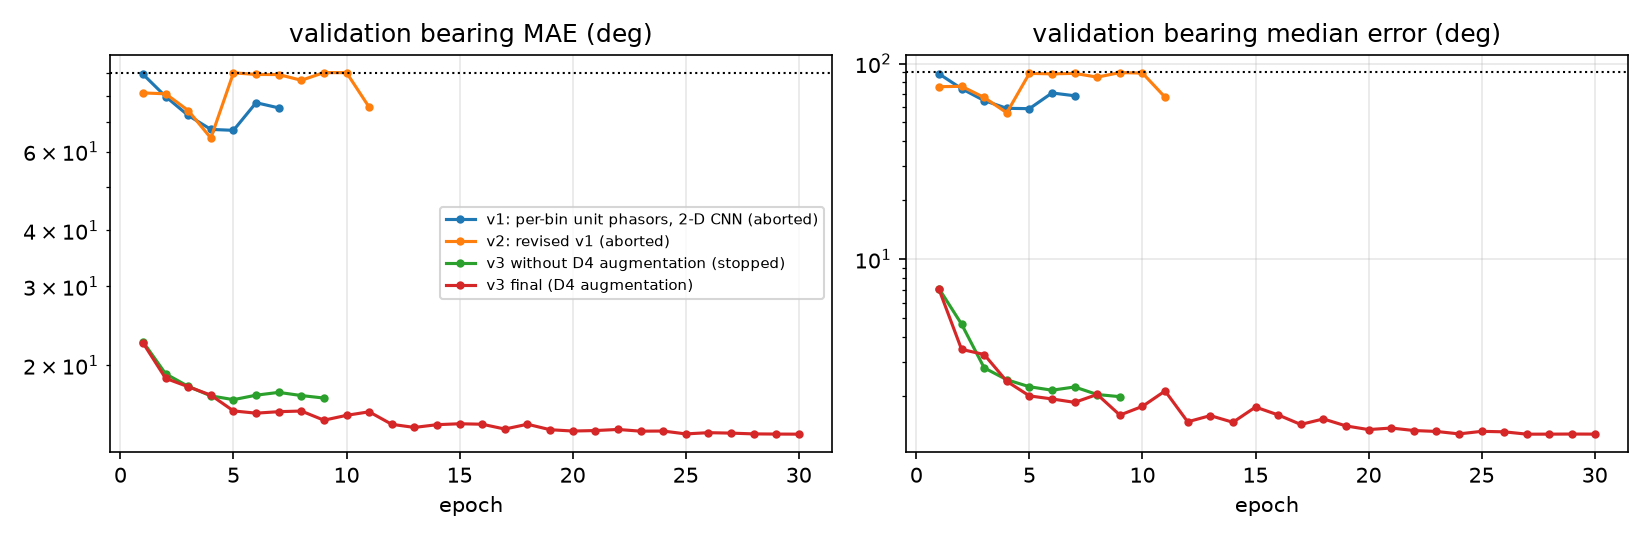
\includegraphics[width=0.85\textwidth]{localizer_design_history.png}
\caption{Validation bearing error of every localizer design we trained, including the two
aborted ones and the stopped run without symmetry augmentation. Dotted line: 90$^\circ$
(chance MAE).}
\label{fig:history}
\end{figure*}

\begin{figure*}[t]
\centering
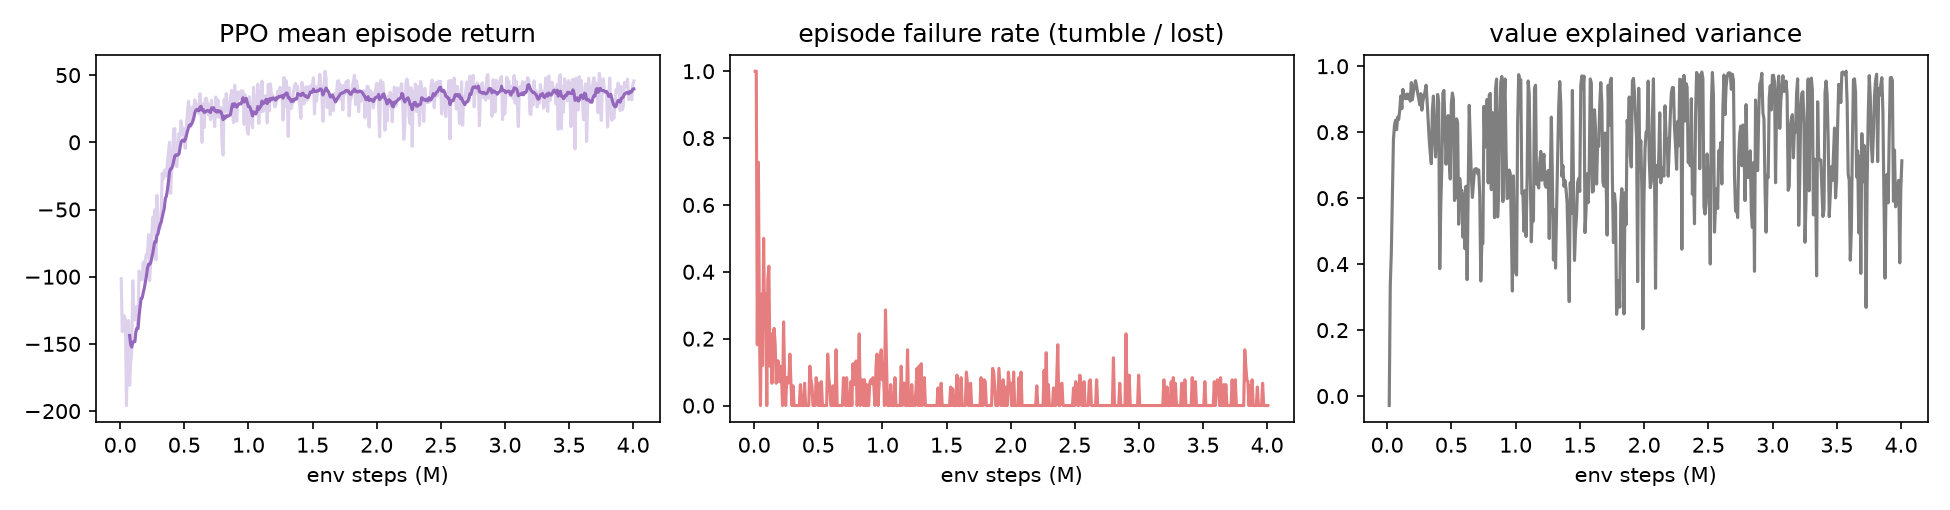
\includegraphics[width=\textwidth]{train_rl.png}
\caption{PPO training, \RLSteps{} steps, \RLEnvs{} parallel environments with random
terrain. Left: mean episode return (light: raw, dark: moving average). Centre: fraction of
episodes ended by a tumble or by losing the person. Right: value-function explained variance.}
\label{fig:trainrl}
\end{figure*}

\begin{figure}[t]
\centering
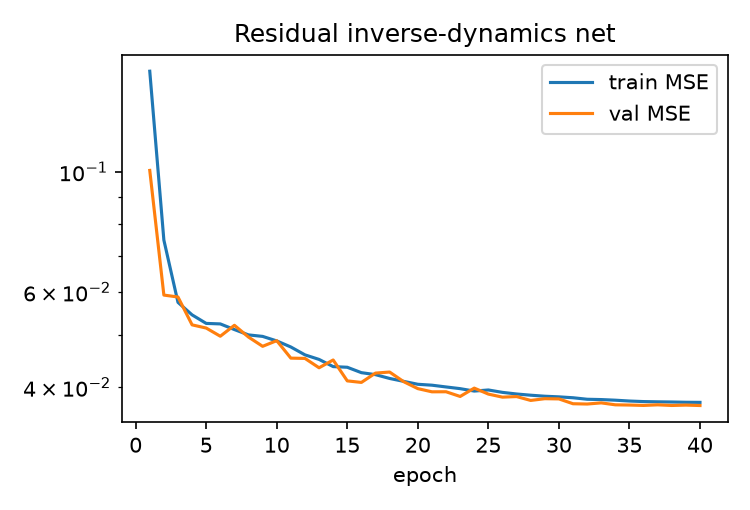
\includegraphics[width=\columnwidth]{train_residual.png}
\caption{Residual inverse-dynamics network, train and validation MSE of the predicted duty.}
\label{fig:trainres}
\end{figure}

\subsection{Localization}

Table~\ref{tab:loc} compares all localizers on the same \NTestSet{} test recordings. The deep
localizer more than halves the classical bearing MAE (\LocdlfullBMAE$^\circ$ against
\LocsrpphatBMAE$^\circ$ for SRP-PHAT and \LocgcclstdoaBMAE$^\circ$ for pairwise GCC-PHAT) and
cuts the median error from \LocsrpphatBMed$^\circ$ to \LocdlfullBMed$^\circ$. Its range MAE
is \LocdlfullRMAE\,m against \LocsrpphatRMAE\,m for matched-filter time of flight. The medians
are close (\LocdlfullRMed{} and \LocsrpphatRMed\,m), so the classical range error comes from a
tail of gross errors where a reflection or noise peak is picked as the first arrival
(Fig.~\ref{fig:loccdf}, right).

The mean bearing error of every method is dominated by low SNR (Fig.~\ref{fig:locsnr}). On the
\SnrAN{} test recordings whose direct-path SNR at the array is below 0\,dB, the deep localizer's
MAE is \LocdlfullSnrABMAE$^\circ$ (SRP-PHAT \LocsrpphatSnrABMAE$^\circ$). From 10 to 20\,dB it is
\LocdlfullSnrCBMAE$^\circ$ (SRP-PHAT \LocsrpphatSnrCBMAE$^\circ$). The mean is therefore a
statement about how often the phone is far, occluded or quiet, more than about the method's
precision.

By front end (Table~\ref{tab:locch}), the ideal channel is easiest (\LocdlfullAusBMAE$^\circ$).
The ultrasonic chirp through the realistic speaker and microphone chain is the hardest
(\LocdlfullBusBMAE$^\circ$, SRP-PHAT \LocsrpphatBusBMAE$^\circ$), because the modelled roll-off
leaves little in-band energy. The 17--19.5\,kHz fallback recovers most of the performance
(\LocdlfullBfbBMAE$^\circ$). By terrain (Table~\ref{tab:locterr}), the deep localizer is best
indoors (\LocdlfullindoorBMAE$^\circ$) and worst on grass (\LocdlfullgrassBMAE$^\circ$), where
ground absorption lowers the SNR. It beats both classical methods on every terrain and channel.

\textbf{Ablations.} Without the phase channels the network is at chance
(\LocdlmagBMAE$^\circ$ MAE, median \LocdlmagBMed$^\circ$), while its range MAE
(\LocdlmagRMAE\,m) is close to that of the full model. This is the expected outcome rather than
a weak baseline. The array's omnidirectional microphones are 10\,cm apart at most, so
level differences between them carry almost no direction, and the inter-channel delays (at most
0.3\,ms, or 14 samples) are invisible in log-power maps with a 32-sample hop. Range survives
because it comes from arrival time. Training without multipath (anechoic training set, normal
test set) raises the bearing MAE from \LocdlfullBMAE$^\circ$ to \LocdlanechoicBMAE$^\circ$ and
the range MAE from \LocdlfullRMAE{} to \LocdlanechoicRMAE\,m. Multipath augmentation helps, but
by less than the input representation does.

\textbf{Latency.} On the \GPU, batched inference costs \LatDlFullBatchedMsPerExample\,ms per
example against \LatClassicalBatchedMsPerExample\,ms for the classical pipeline. A single
example takes \LatDlFullSingleMsGpu\,ms on the GPU and \LatDlFullSingleMsCpu\,ms on the CPU, close
to the 50\,ms chirp period. These timings were taken while a closed-loop evaluation shared the
GPU, so they are upper bounds.

\begin{table*}[t]
\centering
\caption{Localization on the \NTestSet{} test recordings (all terrains and channels).}
\label{tab:loc}
\begin{tabular}{lrrrrrrrr}
\toprule
method & \multicolumn{5}{c}{bearing error (deg)} & \multicolumn{3}{c}{range error (m)}\\
\cmidrule(lr){2-6}\cmidrule(lr){7-9}
 & MAE & RMSE & median & p90 & \% $<10^\circ$ & MAE & RMSE & median\\
\midrule
SRP-PHAT & 23.3 & 45.8 & 5.1 & 80.3 & 55 & 0.69 & 1.77 & 0.09 \\
GCC-PHAT LS-TDOA & 25.2 & 48.6 & 6.1 & 92.0 & 61 & 0.69 & 1.77 & 0.09 \\
DL (mag.+phase) & 13.2 & 34.4 & 1.3 & 38.5 & 78 & 0.12 & 0.32 & 0.06 \\
DL (magnitude only) & 89.3 & 103.1 & 89.0 & 160.9 & 5 & 0.14 & 0.36 & 0.07 \\
DL (no multipath in training) & 15.8 & 37.6 & 2.0 & 46.0 & 73 & 0.15 & 0.35 & 0.08 \\
\bottomrule
\end{tabular}

\end{table*}

\begin{table*}[t]
\centering
\caption{Bearing MAE / median (deg) by front-end channel, same test set.}
\label{tab:locch}
\begin{tabular}{lrrr}
\toprule
method & A\_us & B\_us & B\_fb\\
\midrule
SRP-PHAT & 14.8 / 3.0 & 61.6 / 45.9 & 19.1 / 2.4 \\
GCC-PHAT LS-TDOA & 16.8 / 4.3 & 61.7 / 44.4 & 21.7 / 5.3 \\
DL (mag.+phase) & 6.3 / 1.0 & 44.4 / 19.6 & 9.9 / 1.1 \\
DL (magnitude only) & 88.8 / 88.1 & 91.1 / 91.8 & 89.2 / 89.0 \\
DL (no multipath in training) & 9.2 / 1.6 & 48.4 / 26.2 & 11.3 / 1.5 \\
\bottomrule
\end{tabular}

\end{table*}

\begin{table*}[t]
\centering
\caption{Bearing MAE / median (deg) by terrain, same test set.}
\label{tab:locterr}
\begin{tabular}{lrrrrrr}
\toprule
method & flat & slope & rough & grass & indoor & obstacles\\
\midrule
SRP-PHAT & 20.5 / 2.2 & 24.0 / 7.2 & 22.7 / 5.3 & 28.7 / 9.6 & 20.0 / 6.4 & 23.6 / 3.0 \\
GCC-PHAT LS-TDOA & 23.5 / 5.0 & 26.4 / 7.0 & 24.3 / 5.7 & 29.0 / 6.3 & 22.1 / 6.7 & 26.0 / 5.9 \\
DL (mag.+phase) & 10.7 / 0.8 & 14.4 / 2.0 & 13.5 / 2.0 & 18.4 / 1.3 & 8.3 / 1.0 & 13.9 / 1.0 \\
DL (magnitude only) & 88.8 / 84.2 & 89.0 / 88.3 & 92.9 / 94.3 & 88.8 / 90.9 & 87.5 / 88.5 & 88.7 / 87.2 \\
DL (no multipath in training) & 14.1 / 1.6 & 17.7 / 3.6 & 15.9 / 2.8 & 18.3 / 1.3 & 12.6 / 1.8 & 16.0 / 1.6 \\
\bottomrule
\end{tabular}

\end{table*}

\begin{figure*}[t]
\centering
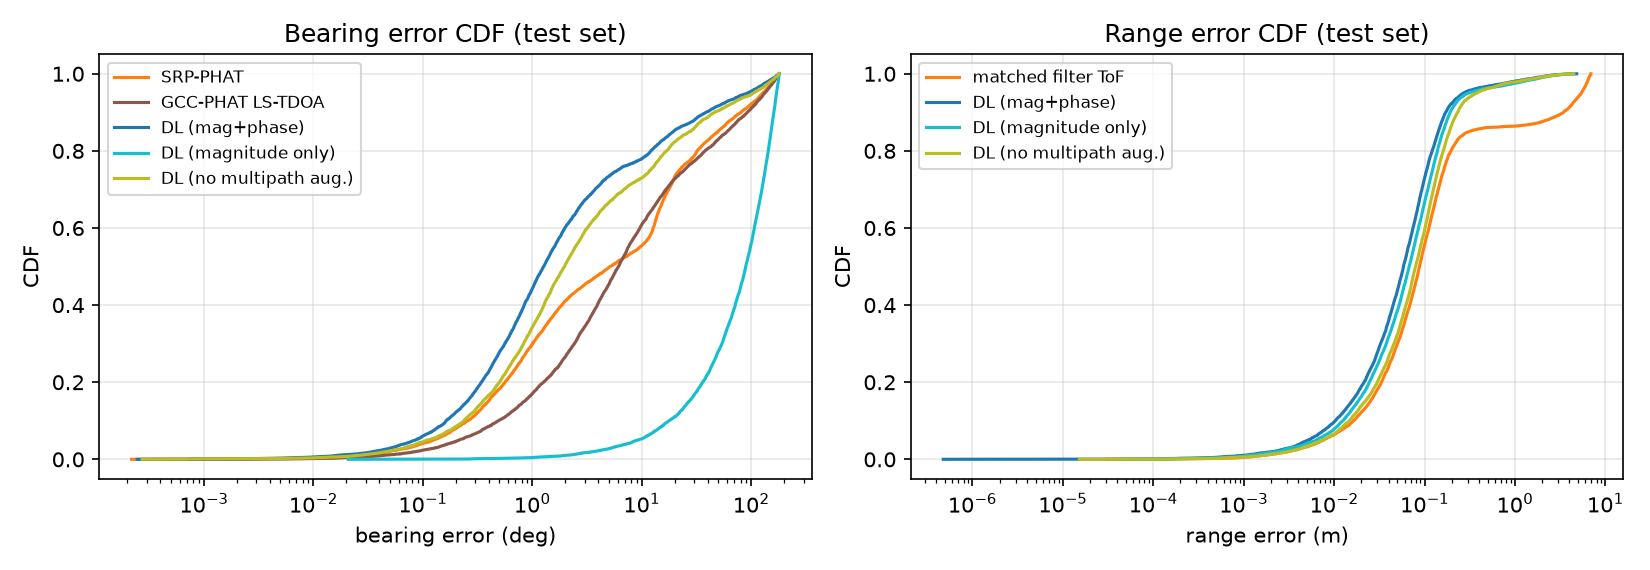
\includegraphics[width=\textwidth]{loc_cdf.png}
\caption{Error CDFs on the test set. Range for SRP-PHAT is the matched-filter time of flight.}
\label{fig:loccdf}
\end{figure*}

\begin{figure*}[t]
\centering
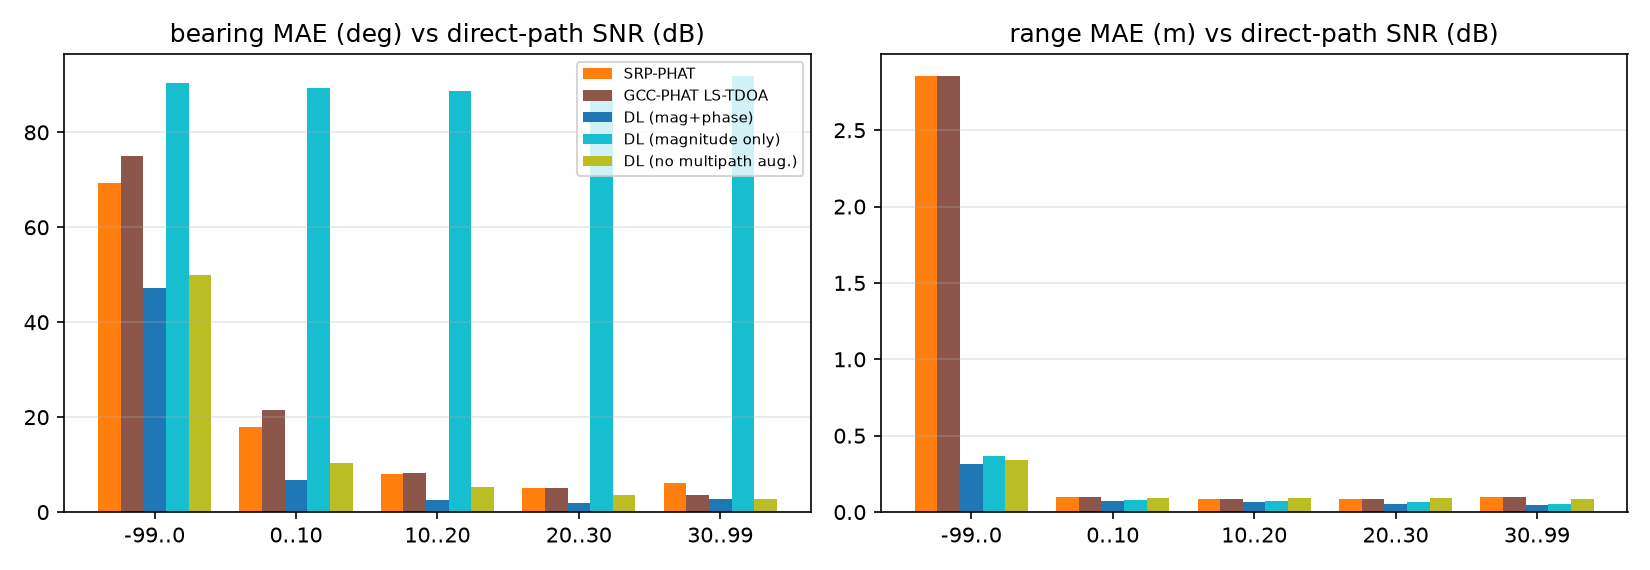
\includegraphics[width=\textwidth]{loc_vs_snr.png}
\caption{Bearing and range MAE by direct-path SNR at the array.}
\label{fig:locsnr}
\end{figure*}

\begin{figure*}[t]
\centering
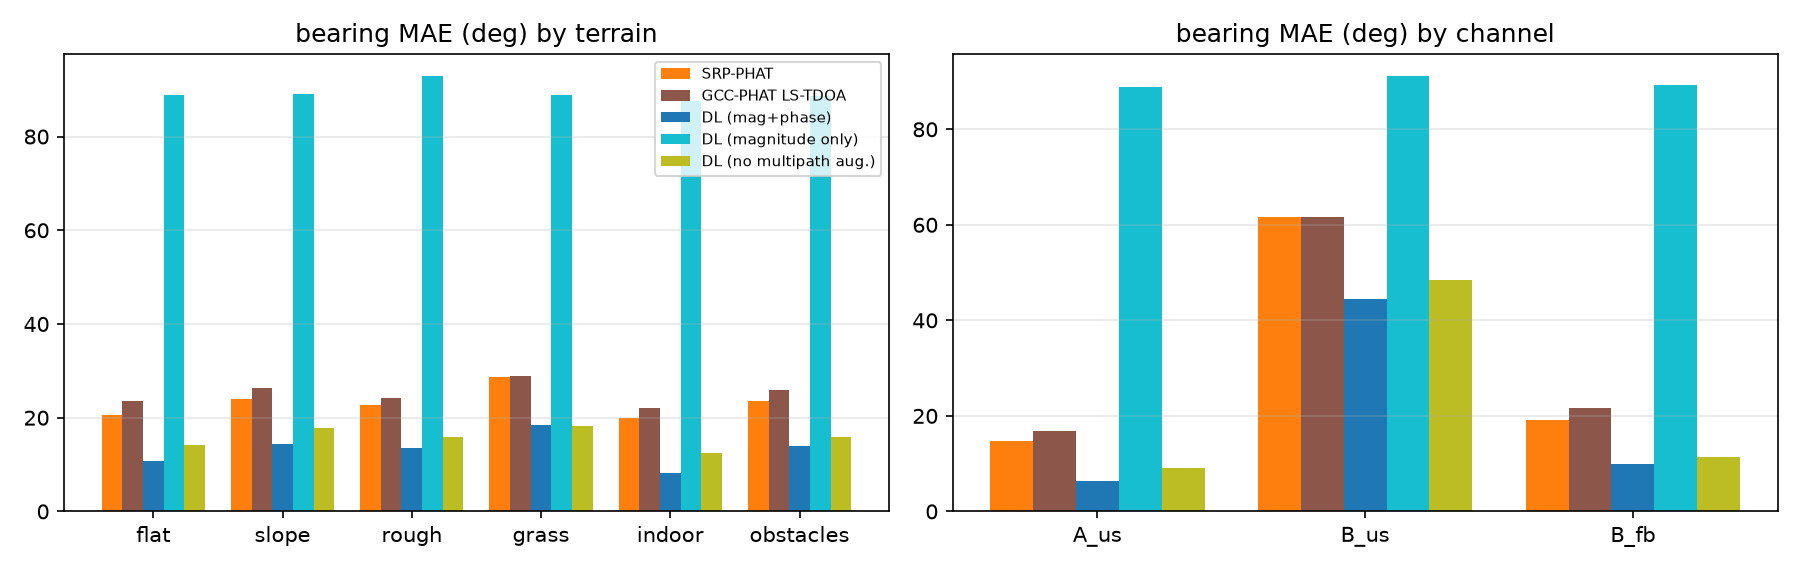
\includegraphics[width=\textwidth]{loc_by_terrain_channel.png}
\caption{Bearing MAE by terrain and by front-end channel.}
\label{fig:locterr}
\end{figure*}

\subsection{Closed-loop following, ideal channel}

Tables~\ref{tab:clsucc}--\ref{tab:clextra} and Fig.~\ref{fig:clbars} give the closed-loop
results on channel A\_us, with \CLAusN{} episodes of \CLAusSeconds\,s per terrain and the
same scenarios for every controller.

\textbf{Localization quality carries through to following where the vehicle is easy to
drive.} On flat, rough, indoor and obstacle terrain, the oracle succeeds in every episode and
the tracker-based controllers come close. The deep localizer keeps the robot nearer to the
person than GCC-PHAT does: pooled mean distance is \CLAusdltrackdist\,m against
\CLAusgcctrackdist\,m, and final distance \CLAusdltrackfinal{} against \CLAusgcctrackfinal\,m. In
closed loop the in-the-loop bearing error is \CLAusdltrackbmae$^\circ$ against
\CLAusgcctrackbmae$^\circ$ (Table~\ref{tab:clbmae}). It is lower than the test-set errors
because the robot keeps the person close and in front.

\textbf{Where the vehicle is hard to drive, control dominates.} On slope and grass even the
oracle succeeds in only \CLAusoraclesuccslope\% and \CLAusoraclesuccgrass\% of episodes, so the
pursuit law, not the localizer, is the bottleneck. The PPO policy is the only controller that
handles slopes (\CLAusrlsuccslope\% success against \CLAusoraclesuccslope\% for the oracle and
\CLAusdltracksuccslope\% for DL + tracker). It is also the best on grass
(\CLAusrlsuccgrass\%), and it does this with the classical acoustic features only. Its pooled
success rate is the highest of all methods (\CLAusrlsucc\% against \CLAusoraclesucc\% for the
oracle). Its control effort (\CLAusrleffort) is close to the oracle's (\CLAusoracleeffort),
and it spends the least time closer than 0.4\,m (\CLAusrlclose\%). On flat ground it trails slightly behind
(\CLAusrldistflat\,m mean distance against \CLAusdltrackdistflat\,m for DL + tracker), as if it
had learned a looser standoff.

\textbf{DL + PID tumbles, and the residual fixes it.} The cascaded PID holds the standoff
tightly on easy terrain, with mean distance \CLAusdlpiddistflat\,m on flat ground. But it
tumbles: \CLAusdlpidtumbles{} tumble steps per episode pooled, and \CLAusdlpidtumblesindoor{}
indoors, where only \CLAusdlpidsuccindoor\% of episodes succeed. With oracle localization
(\DbgN{} scenarios, \DbgSeconds\,s, \texttt{results/debug\_pid\_indoor.json}) it does not
tumble indoors, but its peak cart pitch reaches \DbgOraclePidindoorPitch\,rad against the
\PitchLimit\,rad limit, against \DbgOraclePursuitindoorPitch\,rad for the pursuit law. Its
duty is saturated \DbgOraclePidindoorSat\% of the time. The inner speed loop
reacts to every stop and start of the person with full duty, and small localization errors over
a 60\,s episode push the cart past the limit. Our PID has no pitch limiter; a practical one
would need it.

Adding the residual raises success indoors to \CLAusdlpidressuccindoor\%, on flat ground to
\CLAusdlpidressuccflat\% and pooled to \CLAusdlpidressucc\% (from \CLAusdlpidsucc\%), and it
cuts tumbles to \CLAusdlpidrestumbles{} per episode. The mechanism is visible with oracle
localization. The residual raises the mean duty but lowers the peak pitch, indoors from
\DbgOraclePidindoorPitch{} to \DbgOraclePidResindoorPitch\,rad and on flat ground from
\DbgOraclePidflatPitch{} to \DbgOraclePidResflatPitch\,rad. Because the feedforward already
supplies the duty the terrain needs, the integrator does less of the work and overshoots less.
The cost is the highest control effort of all methods (\CLAusdlpidreseffort). On slopes neither
PID variant works (\CLAusdlpidsuccslope\% and \CLAusdlpidressuccslope\%). On grass both beat the
pursuit law (\CLAusdlpidsuccgrass\% against \CLAusdltracksuccgrass\% for DL + tracker), because
their integrators make up for the higher rolling resistance.

\textbf{Grass is limited by sensing at range as well.} On grass every controller except the
oracle falls behind late in the episodes (Fig.~\ref{fig:cldist}). Ground absorption lowers the
SNR as the distance grows, the localizer degrades, and the robot loses ground. The DL bearing
error in the loop is \CLAusdltrackbmaegrass$^\circ$ on grass against
\CLAusdltrackbmaeflat$^\circ$ on flat ground.

\begin{table*}[t]
\centering
\caption{Follow success rate (\%), channel A\_us, \CLAusN{} episodes per terrain. Success:
within \FollowRadius\,m of the person for at least \SuccessFrac\% of the time after a \WarmupS\,s
warm-up, and no tumble.}
\label{tab:clsucc}
\begin{tabular}{lrrrrrrr}
\toprule
method & flat & slope & rough & grass & indoor & obstacles & all\\
\midrule
Oracle + pursuit & 100 & 50 & 100 & 30 & 100 & 100 & 80 \\
GCC-PHAT + tracker & 97 & 17 & 93 & 17 & 100 & 97 & 70 \\
DL + tracker & 97 & 37 & 100 & 20 & 100 & 93 & 74 \\
DL + PID & 80 & 13 & 87 & 47 & 23 & 87 & 56 \\
DL + PID + residual & 100 & 17 & 93 & 47 & 97 & 100 & 76 \\
RL (PPO) & 93 & 93 & 97 & 63 & 100 & 97 & 91 \\
\bottomrule
\end{tabular}

\end{table*}

\begin{table*}[t]
\centering
\caption{Mean distance to the person after warm-up (m), channel A\_us. The standoff is
\Standoff\,m.}
\label{tab:cldist}
\begin{tabular}{lrrrrrrr}
\toprule
method & flat & slope & rough & grass & indoor & obstacles & all\\
\midrule
Oracle + pursuit & 0.85 & 1.34 & 0.94 & 1.51 & 0.80 & 0.86 & 1.05 \\
GCC-PHAT + tracker & 1.29 & 3.95 & 1.34 & 2.27 & 0.88 & 1.09 & 1.80 \\
DL + tracker & 1.20 & 2.01 & 0.95 & 1.84 & 0.82 & 0.97 & 1.30 \\
DL + PID & 0.84 & 4.58 & 0.86 & 1.51 & 0.81 & 0.84 & 1.57 \\
DL + PID + residual & 0.82 & 4.26 & 0.85 & 1.54 & 0.80 & 0.82 & 1.52 \\
RL (PPO) & 1.39 & 2.15 & 1.22 & 1.92 & 0.80 & 1.01 & 1.41 \\
\bottomrule
\end{tabular}

\end{table*}

\begin{table*}[t]
\centering
\caption{Control effort, mean $u^2$ over both wheels, channel A\_us.}
\label{tab:cleffort}
\begin{tabular}{lrrrrrrr}
\toprule
method & flat & slope & rough & grass & indoor & obstacles & all\\
\midrule
Oracle + pursuit & 0.197 & 0.425 & 0.262 & 0.499 & 0.189 & 0.208 & 0.297 \\
GCC-PHAT + tracker & 0.225 & 0.546 & 0.281 & 0.475 & 0.206 & 0.239 & 0.329 \\
DL + tracker & 0.211 & 0.505 & 0.273 & 0.504 & 0.190 & 0.221 & 0.317 \\
DL + PID & 0.328 & 0.669 & 0.365 & 0.603 & 0.295 & 0.335 & 0.433 \\
DL + PID + residual & 0.428 & 0.718 & 0.466 & 0.670 & 0.390 & 0.435 & 0.518 \\
RL (PPO) & 0.216 & 0.377 & 0.281 & 0.521 & 0.200 & 0.230 & 0.304 \\
\bottomrule
\end{tabular}

\end{table*}

\begin{table*}[t]
\centering
\caption{Bearing error of the localizer in the loop (deg), channel A\_us. RL has no explicit
bearing estimate.}
\label{tab:clbmae}
\begin{tabular}{lrrrrrrr}
\toprule
method & flat & slope & rough & grass & indoor & obstacles & all\\
\midrule
Oracle + pursuit & 0.0 & 0.0 & 0.0 & 0.0 & 0.0 & 0.0 & 0.0 \\
GCC-PHAT + tracker & 10.0 & 12.9 & 10.0 & 14.3 & 7.7 & 9.1 & 10.7 \\
DL + tracker & 4.3 & 4.1 & 1.6 & 7.4 & 1.7 & 3.8 & 3.8 \\
DL + PID & 1.5 & 6.0 & 2.5 & 7.2 & 2.2 & 1.6 & 3.5 \\
DL + PID + residual & 1.4 & 10.2 & 2.2 & 7.4 & 1.8 & 1.5 & 4.1 \\
RL (PPO) & -- & -- & -- & -- & -- & -- & -- \\
\bottomrule
\end{tabular}

\end{table*}

\begin{table*}[t]
\centering
\caption{Further metrics, channel A\_us, pooled over all terrains and episodes.}
\label{tab:clextra}
\begin{tabular}{lrrrrrrrr}
\toprule
method & \% time within & final dist. & time to reach & path & person path & collision & tumbles & \% time\\
 & radius & (m) & radius (s) & (m) & (m) & steps & /episode & $<0.4$ m\\
\midrule
Oracle + pursuit & 90 & 1.05 & 3.9 & 29.4 & 27.3 & 2.0 & 0.00 & 1.5 \\
GCC-PHAT + tracker & 80 & 2.87 & 4.7 & 32.7 & 27.3 & 2.3 & 0.04 & 1.7 \\
DL + tracker & 85 & 1.55 & 4.2 & 30.8 & 27.3 & 3.0 & 0.17 & 1.6 \\
DL + PID & 86 & 2.74 & 4.1 & 35.6 & 27.3 & 2.1 & 2.51 & 1.3 \\
DL + PID + residual & 84 & 2.58 & 4.2 & 35.0 & 27.3 & 1.9 & 0.03 & 1.3 \\
RL (PPO) & 93 & 1.90 & 3.8 & 28.1 & 27.3 & 2.7 & 0.00 & 0.7 \\
\bottomrule
\end{tabular}

\end{table*}

\begin{figure*}[t]
\centering
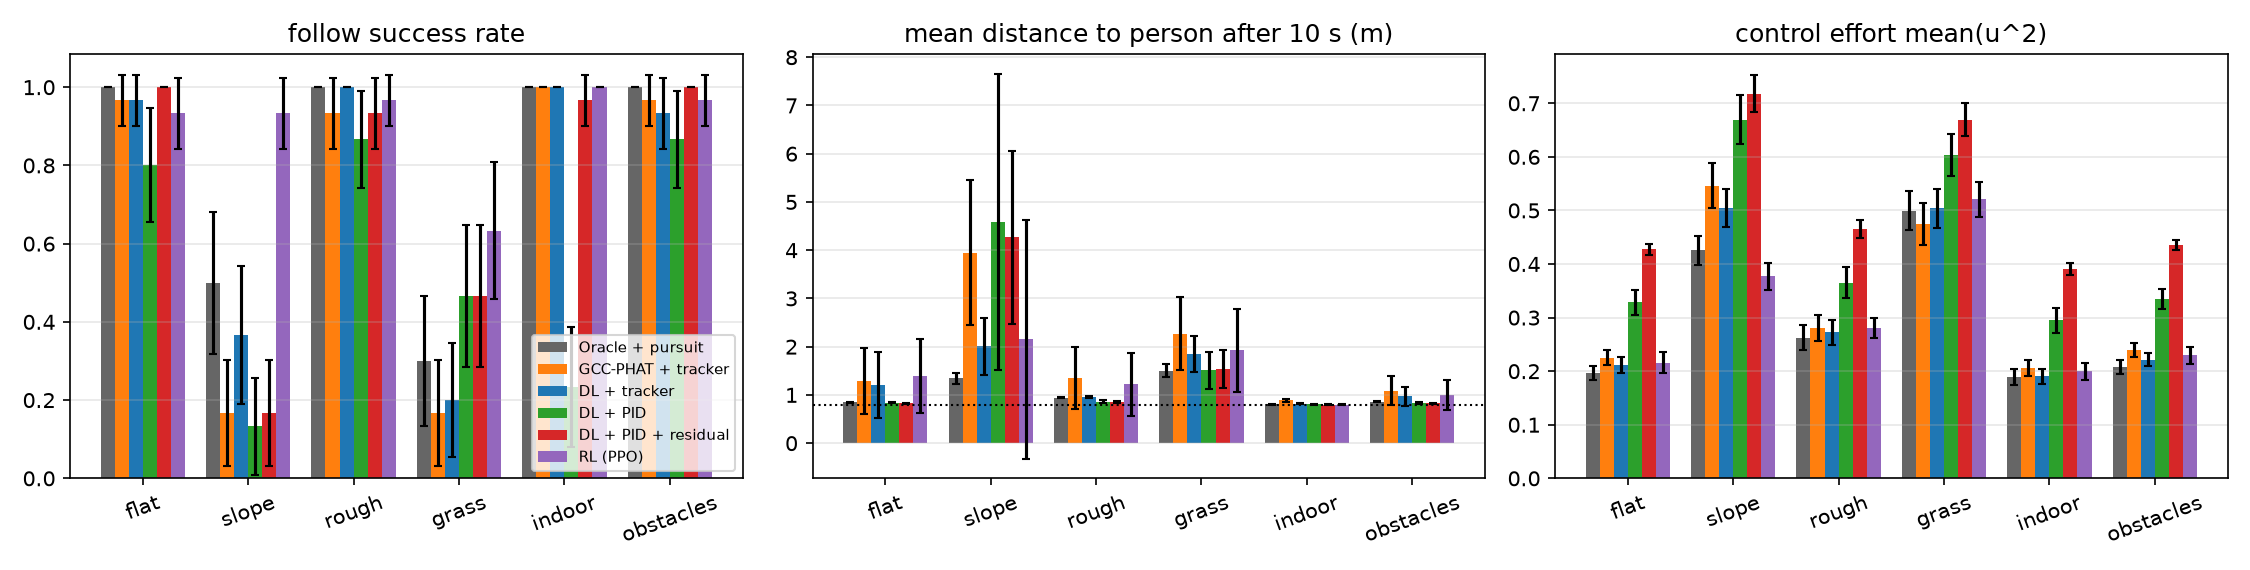
\includegraphics[width=\textwidth]{closed_loop_bars_A_us.png}
\caption{Closed-loop results on channel A\_us. Error bars: 95\% intervals over \CLAusN{} episodes.}
\label{fig:clbars}
\end{figure*}

\begin{figure*}[t]
\centering
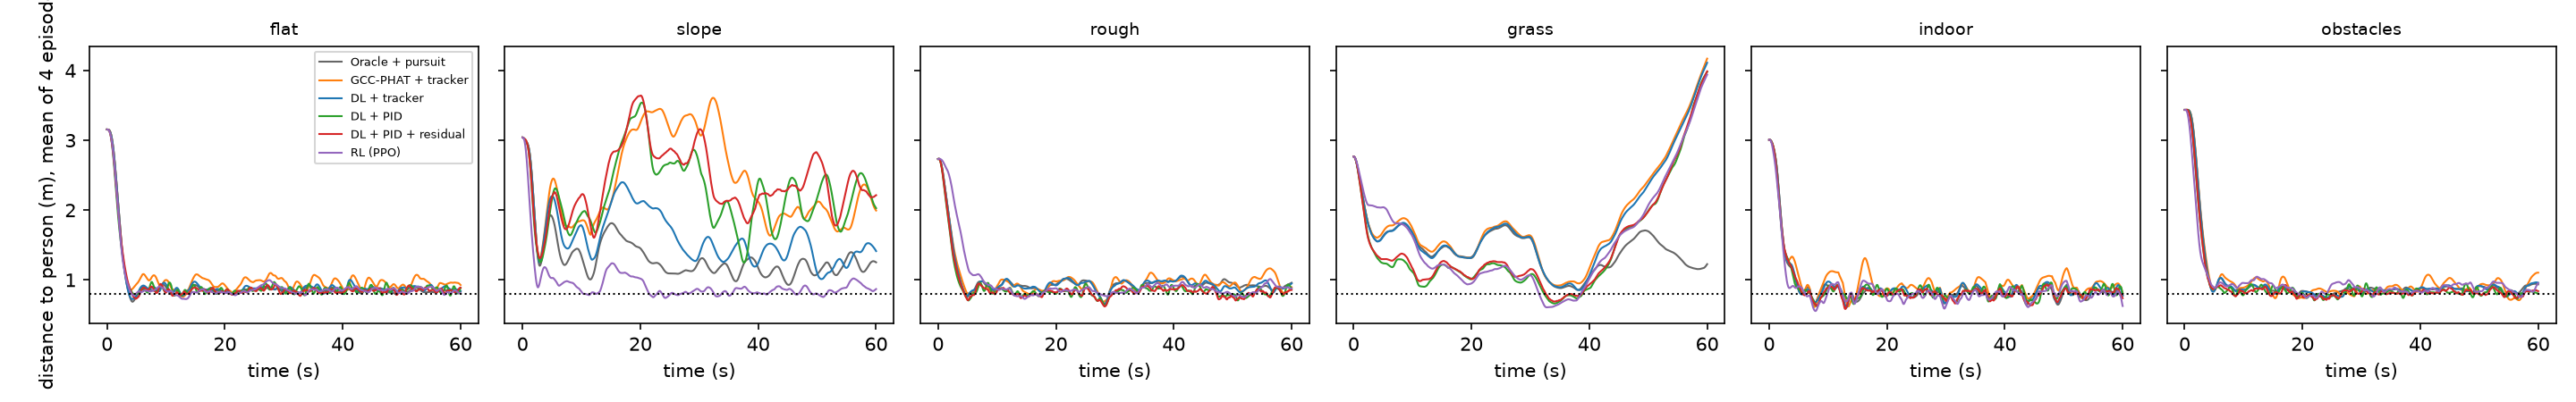
\includegraphics[width=\textwidth]{distance_curves_A_us.png}
\caption{Distance to the person over time, mean of the first four episodes per terrain,
channel A\_us. Dotted: standoff.}
\label{fig:cldist}
\end{figure*}

\begin{figure*}[t]
\centering
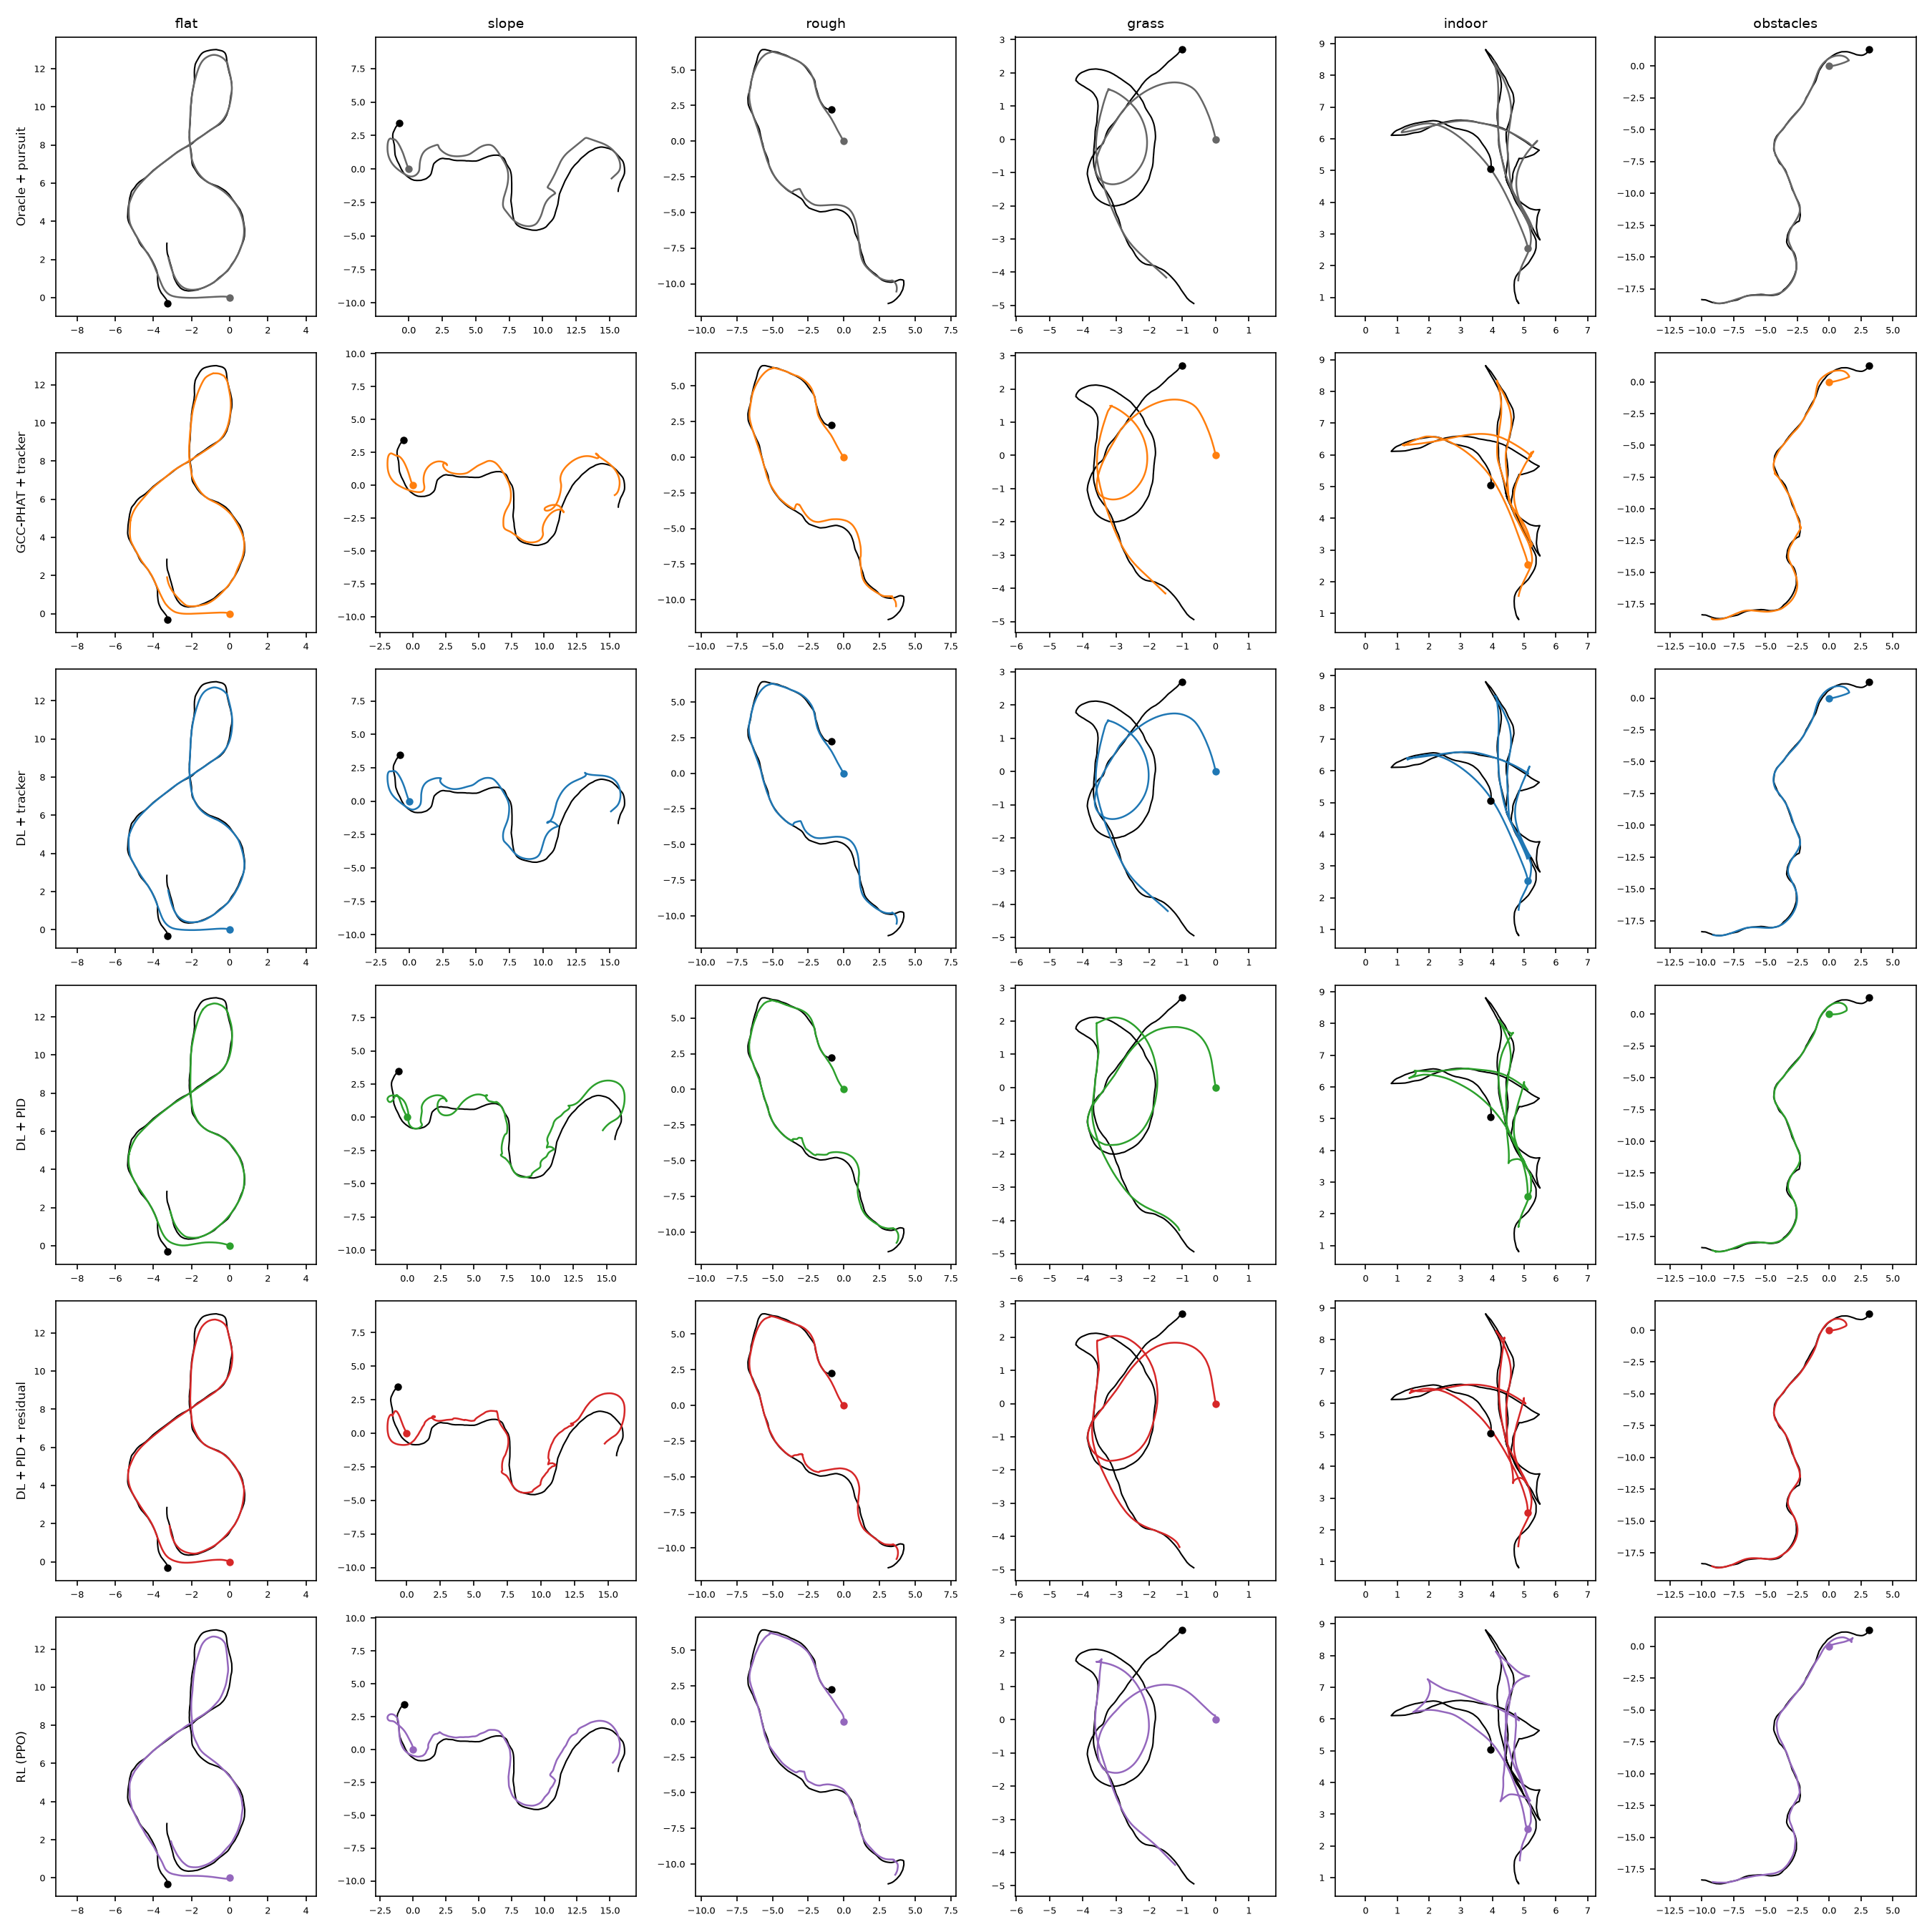
\includegraphics[width=\textwidth]{trajectories_A_us.png}
\caption{First-episode trajectories per controller (rows) and terrain (columns), channel
A\_us. Black: person; colour: robot; dots: start.}
\label{fig:cltraj}
\end{figure*}

\begin{figure}[t]
\centering
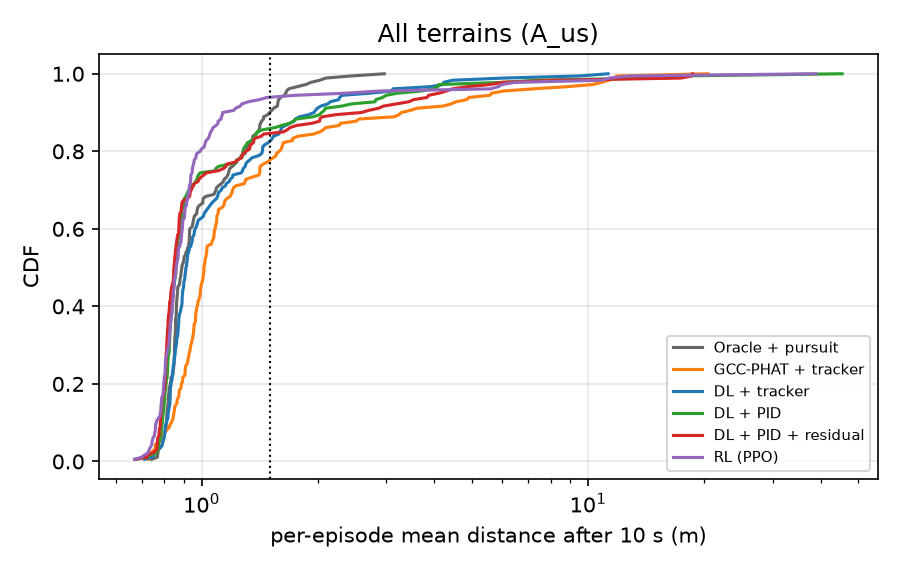
\includegraphics[width=\columnwidth]{closed_loop_cdf_A_us.png}
\caption{CDF of the per-episode mean distance, all terrains, channel A\_us. Dotted: follow
radius.}
\label{fig:clcdf}
\end{figure}

\subsection{Closed-loop following, realistic channel with fallback chirp}

Table~\ref{tab:bfbsucc} repeats the evaluation on channel B\_fb (realistic front end, 17--19.5\,kHz
chirp) with the same scenarios. The deep localizer was trained on all three channels. The RL
policy was trained only on A\_us, so B\_fb is out of distribution for it.

The realistic front end widens the gap between the localizers. In the loop, GCC-PHAT's bearing
error rises to \CLBfbgcctrackbmae$^\circ$ (from \CLAusgcctrackbmae$^\circ$ on A\_us), while the
deep localizer's rises only to \CLBfbdltrackbmae$^\circ$ (from \CLAusdltrackbmae$^\circ$). DL +
tracker keeps its success rate (\CLBfbdltracksucc\% pooled, \CLAusdltracksucc\% on A\_us) and
GCC-PHAT + tracker drops to \CLBfbgcctracksucc\%, with a final distance of
\CLBfbgcctrackfinal\,m against \CLBfbdltrackfinal\,m. DL + PID + residual reaches
\CLBfbdlpidressucc\%. It is again far more reliable than DL + PID (\CLBfbdlpidsucc\%,
\CLBfbdlpidtumbles{} tumble steps per episode against \CLBfbdlpidrestumbles). PPO, out of
distribution, falls from \CLAusrlsucc\% to \CLBfbrlsucc\%. It is still the best controller on
slopes (\CLBfbrlsuccslope\%) and grass (\CLBfbrlsuccgrass\%), but it is no longer the best on
flat ground (\CLBfbrlsuccflat\% against \CLBfbdltracksuccflat\% for DL + tracker), and its
final distance (\CLBfbrlfinal\,m) is the second largest after GCC-PHAT. With realistic
hardware, a policy trained on the features of one front end loses part of its advantage, and
better sensing becomes more valuable.

\begin{table*}[t]
\centering
\caption{Follow success rate (\%), channel B\_fb, \CLBfbN{} episodes per terrain.}
\label{tab:bfbsucc}
\begin{tabular}{lrrrrrrr}
\toprule
method & flat & slope & rough & grass & indoor & obstacles & all\\
\midrule
Oracle + pursuit & 100 & 50 & 100 & 30 & 100 & 100 & 80 \\
GCC-PHAT + tracker & 83 & 20 & 83 & 17 & 97 & 90 & 65 \\
DL + tracker & 97 & 37 & 100 & 23 & 100 & 100 & 76 \\
DL + PID & 60 & 13 & 77 & 47 & 30 & 87 & 52 \\
DL + PID + residual & 100 & 20 & 97 & 50 & 100 & 97 & 77 \\
RL (PPO) & 80 & 77 & 87 & 57 & 97 & 87 & 81 \\
\bottomrule
\end{tabular}

\end{table*}

\begin{table*}[t]
\centering
\caption{Mean distance after warm-up (m), channel B\_fb.}
\label{tab:bfbdist}
\begin{tabular}{lrrrrrrr}
\toprule
method & flat & slope & rough & grass & indoor & obstacles & all\\
\midrule
Oracle + pursuit & 0.85 & 1.34 & 0.94 & 1.51 & 0.80 & 0.86 & 1.05 \\
GCC-PHAT + tracker & 2.01 & 7.72 & 1.61 & 3.09 & 0.94 & 1.65 & 2.84 \\
DL + tracker & 1.21 & 2.23 & 0.95 & 2.29 & 0.82 & 0.87 & 1.40 \\
DL + PID & 1.19 & 5.63 & 0.86 & 1.57 & 0.81 & 0.84 & 1.82 \\
DL + PID + residual & 0.83 & 3.85 & 0.85 & 1.52 & 0.80 & 0.83 & 1.45 \\
RL (PPO) & 2.20 & 5.39 & 2.01 & 2.59 & 0.86 & 1.79 & 2.47 \\
\bottomrule
\end{tabular}

\end{table*}

\begin{table*}[t]
\centering
\caption{Further metrics, channel B\_fb, pooled over all terrains and episodes.}
\label{tab:bfbextra}
\begin{tabular}{lrrrrrrrr}
\toprule
method & \% time within & final dist. & time to reach & path & person path & collision & tumbles & \% time\\
 & radius & (m) & radius (s) & (m) & (m) & steps & /episode & $<0.4$ m\\
\midrule
Oracle + pursuit & 90 & 1.05 & 3.9 & 29.4 & 27.3 & 2.0 & 0.00 & 1.5 \\
GCC-PHAT + tracker & 74 & 4.49 & 5.2 & 31.7 & 27.3 & 2.0 & 0.07 & 1.7 \\
DL + tracker & 85 & 1.93 & 4.5 & 31.1 & 27.3 & 2.9 & 0.00 & 1.6 \\
DL + PID & 85 & 3.18 & 4.2 & 36.0 & 27.3 & 2.6 & 2.57 & 1.2 \\
DL + PID + residual & 85 & 2.03 & 4.0 & 34.6 & 27.3 & 1.8 & 0.07 & 1.4 \\
RL (PPO) & 85 & 3.67 & 4.3 & 29.1 & 27.3 & 3.8 & 0.00 & 0.7 \\
\bottomrule
\end{tabular}

\end{table*}

\begin{figure*}[t]
\centering
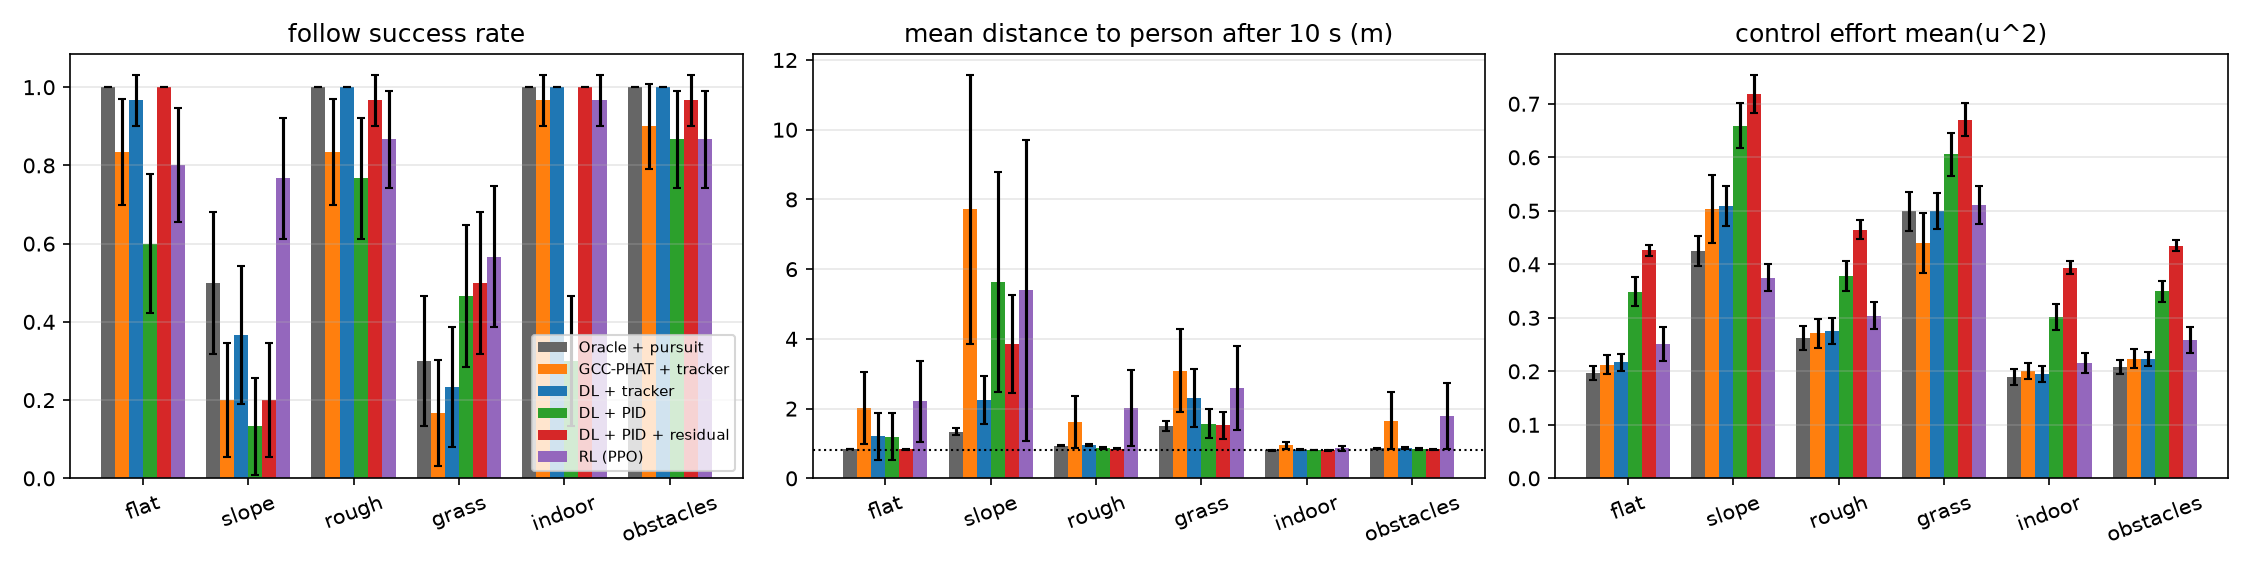
\includegraphics[width=\textwidth]{closed_loop_bars_B_fb.png}
\caption{Closed-loop results on channel B\_fb. Error bars: 95\% intervals over \CLBfbN{} episodes.}
\label{fig:bfbbars}
\end{figure*}

\section{Discussion}
\label{sec:discussion}

\textbf{What the deep localizer adds.} At this aperture and frequency the classical estimators
are not imprecise; their median errors are a few degrees. Their problem is a heavy tail of
wrong peaks: aliased lobes, reflections and noise when the direct path is weak. The deep model
inherits the steered response through its initialisation and learns which frames and which
lobes to trust. It halves the mean error and cuts range gross errors sharply, but it does not
remove the low-SNR tail (Fig.~\ref{fig:locsnr}). In closed loop the gain shows up as tighter
following on easy terrain, not as more successes.

\textbf{The comparison of controllers is confounded in two ways.} First, RL sees classical
acoustic features and the other learned controllers see the deep localizer, so RL's lead says
that a learned policy can compensate for poorer sensing with better driving, not that RL beats
deep localization. An RL policy on top of the deep localizer is the obvious next experiment,
and we did not run it. Second, our PID and pursuit gains were tuned by hand, and our PID lacks
a pitch limiter. A better-tuned classical controller would narrow the gap on slopes, but we have
not shown by how much. RL was trained on the simulator it is tested in, with randomised
terrain parameters but the same model. Against a real sphere it may lose more than the
model-based controllers, whose structure does not depend on the simulator.

\textbf{What the residual learned.} It learned how much duty, beyond what the flat-ground mixer
assumes, the current terrain needs to hold the current motion. It infers the terrain from the
last 0.5\,s of duties and proprioception and never sees a label. It helps where the inner loop
otherwise has to integrate a large load, and it smooths the cart's pitch. It does not make
slopes work: there the problem is the downhill drift and the cart's pitch limit, which no
feedforward on speed and yaw rate can fix.

\section{Limitations}

Everything is simulated. The acoustic model has no diffraction, no speaker directivity, no
body shadowing by the person carrying the phone, no wind, and no motor or rolling noise from
the robot itself, which would sit in the same band. The INMP441 response above 20\,kHz and the
decimation filter edges come from our model, not from measurement. Many phones do not emit
energy above 20\,kHz at all, which is why we report the fallback chirp, and that chirp is
audible to some people. Range depends on an emission schedule shared by phone and robot, which
we assume (100\,$\mu$s jitter, $\pm$200\,$\mu$s bias) but did not build. Without it only
bearing is available.

The sphere is modelled as planar pitch dynamics with a separate lateral pendulum and
first-order yaw, rolling without slip, and an inelastic wall contact. It is not a 3-D contact
model, and its parameters are not identified from a real robot. The simulator applies duties
up to 1.0 with no slew limit, while the firmware clamps to 0.8 and limits the slew to 4 per
second, so the deployed system is slower than the simulated one.

The residual network's design error was found with the oracle diagnostic, which runs on the
first \DbgN{} evaluation scenarios of four terrains (\DbgSeconds\,s each). Design decisions made
with this diagnostic, the residual fix in particular, were therefore not made on held-out
scenarios. The problem first showed up in the closed-loop evaluation itself: DL + PID + residual
succeeded in 2 of 30 flat episodes, with 16.6 tumble steps per episode
(\texttt{results/superseded\_closed\_loop\_A\_us\_run1.log}). We fixed the residual, discarded those rows and reran that controller on all
terrains. No other controller was changed after the evaluation started. The PPO run is a single seed. The localizer's best validation
epoch was its last, so it had not fully converged. Each closed-loop configuration was run once
with \CLAusN{} episodes. The 95\% intervals cover scenario variation, not training variation.

No result here is comparable to Daredevil \cite{constandache2014daredevil} or MilliSonic
\cite{wang2019millisonic}. Those systems were measured on hardware, with different signals,
geometries and goals.

\section{Conclusion}

In simulation, a localizer that starts from the SRP-PHAT steering of the actual array and
learns to weight frames halves the classical bearing MAE (\LocdlfullBMAE$^\circ$ against
\LocsrpphatBMAE$^\circ$) and cuts the range MAE from \LocsrpphatRMAE{} to \LocdlfullRMAE\,m on
the same \NTestSet{} test recordings. Phase is essential, since the magnitude-only model is at
chance. Multipath augmentation helps modestly. In closed loop, localization matters most on
easy terrain, while on slopes and grass the controller is the bottleneck: a PPO policy with
classical features was the most reliable follower (\CLAusrlsucc\% pooled success on the ideal
channel), and a learned terrain residual turned a tumbling cascaded PID into a reliable one on
flat, indoor and obstacle terrain. With a realistic front end and the 17--19.5\,kHz fallback
chirp, the deep localizer's closed-loop advantage grows (\CLBfbdltracksucc\% against
\CLBfbgcctracksucc\% success with the same tracker) and PPO's shrinks (\CLBfbrlsucc\%). The firmware and companion app implement the same command
protocol, but whether any of this holds on a real sphere with a real phone is untested.

